\usepackage{tikz}
\usetikzlibrary{automata, positioning, arrows.meta, fit, backgrounds}

\begin{figure}[t]
\centering
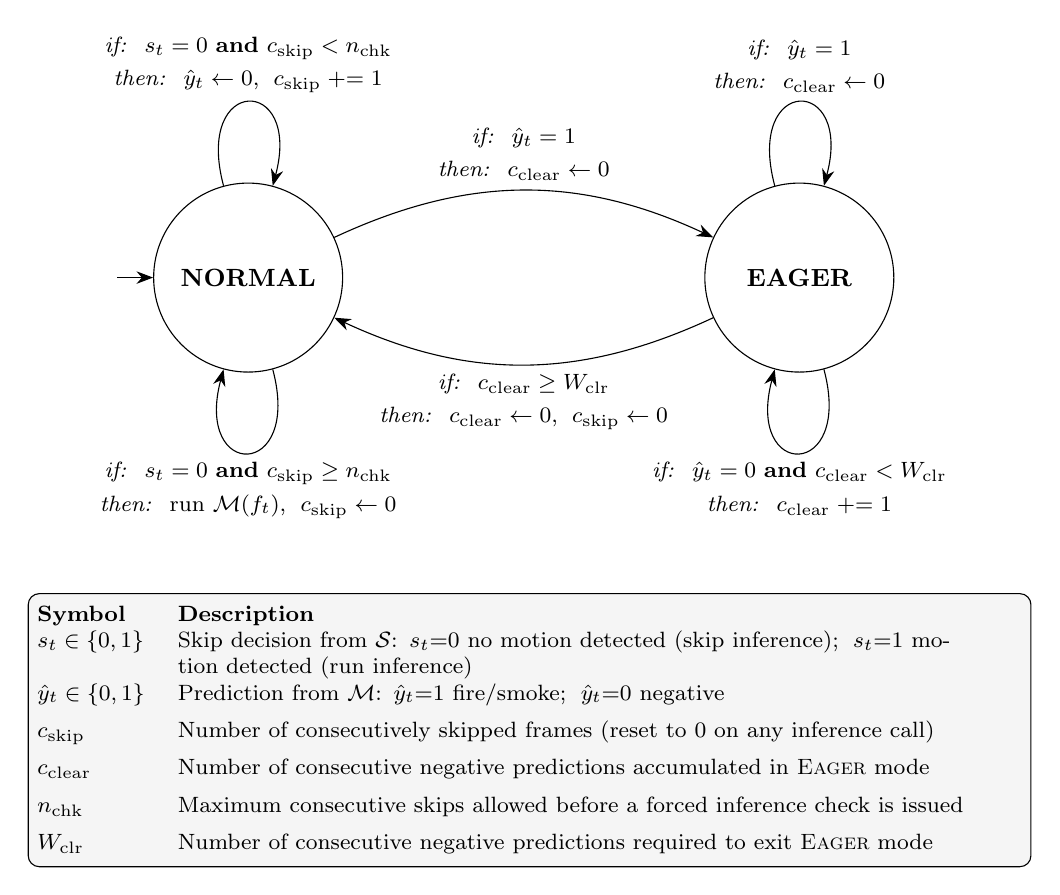
\begin{tikzpicture}[
    node distance=7cm,
    every state/.style={draw, rounded corners, minimum width=2.4cm,
                        minimum height=1.2cm, font=\small\bfseries},
    >={Stealth[length=6pt]},
    auto,
    label style/.style={font=\footnotesize, align=center}
]

%% ── States ───────────────────────────────────────────────────────
\node[state, initial, initial text={}] (normal) {NORMAL};
\node[state, right of=normal]          (eager)  {EAGER};

%% ── NORMAL → EAGER ───────────────────────────────────────────────
%% guard / action
\draw[->] (normal) edge[bend left=25]
    node[above, align=center]{%
        \footnotesize \textit{if:}\; $\hat{y}_t = 1$\\
        \footnotesize \textit{then:}\; $c_{\mathrm{clear}} \leftarrow 0$}
    (eager);

%% ── EAGER → NORMAL ───────────────────────────────────────────────
\draw[->] (eager) edge[bend left=25]
    node[below, align=center]{%
        \footnotesize \textit{if:}\; $c_{\mathrm{clear}} \geq W_{\mathrm{clr}}$\\
        \footnotesize \textit{then:}\; $c_{\mathrm{clear}} \leftarrow 0$,\;
                                         $c_{\mathrm{skip}} \leftarrow 0$}
    (normal);

%% ── NORMAL self-loop: SKIP ───────────────────────────────────────
\draw[->] (normal) edge[loop above, looseness=6]
    node[above, align=center]{%
        \footnotesize \textit{if:}\;
            $s_t = 0$ \textbf{and} $c_{\mathrm{skip}} < n_{\mathrm{chk}}$\\
        \footnotesize \textit{then:}\;
            $\hat{y}_t \leftarrow 0$,\;
            $c_{\mathrm{skip}} \mathrel{+}= 1$}
    (normal);

%% ── NORMAL self-loop: FORCED CHECK ──────────────────────────────
\draw[->] (normal) edge[loop below, looseness=6]
    node[below, align=center]{%
        \footnotesize \textit{if:}\;
            $s_t = 0$ \textbf{and} $c_{\mathrm{skip}} \geq n_{\mathrm{chk}}$\\
        \footnotesize \textit{then:}\;
            run $\mathcal{M}(f_t)$,\;
            $c_{\mathrm{skip}} \leftarrow 0$}
    (normal);

%% ── EAGER self-loop: fire continues ─────────────────────────────
\draw[->] (eager) edge[loop above, looseness=6]
    node[above, align=center]{%
        \footnotesize \textit{if:}\; $\hat{y}_t = 1$\\
        \footnotesize \textit{then:}\; $c_{\mathrm{clear}} \leftarrow 0$}
    (eager);

%% ── EAGER self-loop: counting clears ────────────────────────────
\draw[->] (eager) edge[loop below, looseness=6]
    node[below, align=center]{%
        \footnotesize \textit{if:}\;
            $\hat{y}_t = 0$ \textbf{and} $c_{\mathrm{clear}} < W_{\mathrm{clr}}$\\
        \footnotesize \textit{then:}\;
            $c_{\mathrm{clear}} \mathrel{+}= 1$}
    (eager);

%% ── Legend ───────────────────────────────────────────────────────
\node[draw, rounded corners, fill=gray!8,
      below=2.8cm of normal, anchor=north west,
      xshift=-2.8cm,
      text width=12.5cm,
      font=\footnotesize] (legend)
{
    % \textbf{Notation} \\[2pt]
    \begin{tabular}{@{}lp{10cm}@{}}
    \textbf{Symbol} & \textbf{Description} \\
    \midrule
    $s_t \in \{0,1\}$       & Skip decision from $\mathcal{S}$:
                            $s_t{=}0$ no motion detected (skip inference);\;
                            $s_t{=}1$ motion detected (run inference) \\[4pt]
    $\hat{y}_t \in \{0,1\}$ & Prediction from $\mathcal{M}$:
                            $\hat{y}_t{=}1$ fire/smoke;\;
                            $\hat{y}_t{=}0$ negative \\[4pt]
    $c_{\mathrm{skip}}$     & Number of consecutively skipped frames
                            (reset to $0$ on any inference call) \\[4pt]
    $c_{\mathrm{clear}}$    & Number of consecutive negative predictions
                            accumulated in \textsc{Eager} mode \\[4pt]
    $n_{\mathrm{chk}}$      & Maximum consecutive skips allowed before
                            a forced inference check is issued \\[4pt]
    $W_{\mathrm{clr}}$      & Number of consecutive negative predictions
                            required to exit \textsc{Eager} mode \\
    % \bottomrule
    \end{tabular}
};

\end{tikzpicture}
\caption{%
    State machine of the eager mode extension.
    Each transition is annotated with a \textit{guard} (condition to fire)
    and an \textit{action} (variable updates on transition).
    In \textsc{Normal} mode, $\mathcal{S}$ gates inference: no-motion frames
    are skipped ($c_{\mathrm{skip}} \mathrel{+}= 1$) until $c_{\mathrm{skip}}
    \geq n_{\mathrm{chk}}$, at which point a forced inference check resets
    $c_{\mathrm{skip}}$.
    Any fire or smoke prediction immediately enters \textsc{Eager} mode,
    bypassing $\mathcal{S}$ and running $\mathcal{M}$ on every frame.
    \textsc{Eager} exits to \textsc{Normal} only after $W_{\mathrm{clr}}$
    consecutive negative predictions confirm the scene is safe.
}
\label{fig:eager_statemachine}
\end{figure}
% \begin{algorithm}[t]
% \caption{Eager Mode Extension for AccMotionDet-based Skip Module}
% \label{alg:eagermode}
% \begin{algorithmic}[1]

% \Require Video stream $\{f_t\}$, classifier $\mathcal{M}$,
%          skip module $\mathcal{S}$ (AccMotionDet),
%          clear window $W_{\mathrm{clr}}$,
%          forced-check interval $n_{\mathrm{chk}}$

% \Ensure Per-frame prediction $\hat{y}_t \in \{0, 1\}$
% \State $\textit{eager} \leftarrow \texttt{False}$
% \State $c_{\mathrm{clear}} \leftarrow 0$
% \State $c_{\mathrm{skip}}  \leftarrow 0$

% \For{each frame $f_t$}

%     \If{$\textit{eager} = \texttt{True}$}
%         \State $\hat{y}_t \leftarrow \mathcal{M}(f_t)$
%         \Comment{always run inference in eager mode}

%     \Else
%         \State $s_t \leftarrow \mathcal{S}(f_t)$

%         \If{$s_t = 0$ \textbf{and} $c_{\mathrm{skip}} < n_{\mathrm{chk}}$}
%             \State $\hat{y}_t \leftarrow 0$
%             \Comment{skip: label as negative}
%             \State $c_{\mathrm{skip}} \leftarrow c_{\mathrm{skip}} + 1$
%             \State \textbf{continue}
%         \Else
%             \State $c_{\mathrm{skip}} \leftarrow 0$
%             \State $\hat{y}_t \leftarrow \mathcal{M}(f_t)$
%         \EndIf
%     \EndIf

%     \If{$\hat{y}_t = 1$}
%         \Comment{any fire/smoke prediction immediately enters eager}
%         \State $c_{\mathrm{clear}} \leftarrow 0$
%         \State $\textit{eager} \leftarrow \texttt{True}$

%     \Else
%         \If{$\textit{eager} = \texttt{True}$}
%             \State $c_{\mathrm{clear}} \leftarrow c_{\mathrm{clear}} + 1$
%             \If{$c_{\mathrm{clear}} \geq W_{\mathrm{clr}}$}
%                 \State $\textit{eager}          \leftarrow \texttt{False}$
%                 \Comment{exit eager mode}
%                 \State $c_{\mathrm{clear}} \leftarrow 0$
%                 \State $c_{\mathrm{skip}}  \leftarrow 0$
%             \EndIf
%         \EndIf
%     \EndIf

% \EndFor

% \end{algorithmic}
% \end{algorithm}

% \begin{algorithm}[t]
% \caption{Eager Mode Extension for AccMotionDet-based Skip Module}
% \label{alg:eagermode}
% \begin{algorithmic}[1]

% \Require Video stream $\{f_t\}$, classifier $\mathcal{M}$,
%          skip module $\mathcal{S}$ (AccMotionDet),
%          confirmation window $K_{\text{confirm}}$,
%          clear window $W_{\text{clr}}$,
%          forced-check interval $n_{\text{chk}}$

% \Ensure Per-frame prediction $\hat{y}_t \in \{0, 1\}$

% \State $\textit{eager} \leftarrow \texttt{False}$
% \State $c_{\text{fire}} \leftarrow 0$ \Comment{consecutive fire/smoke prediction count}
% \State $c_{\text{clear}} \leftarrow 0$ \Comment{consecutive negative prediction count}
% \State $c_{\text{skip}} \leftarrow 0$ \Comment{consecutive skipped frame count}

% \For{each frame $f_t$}

%     \If{$\textit{eager} = \texttt{True}$}
%         \State $\hat{y}_t \leftarrow \mathcal{M}(f_t)$ \Comment{always run inference in eager mode}
%     \Else
%         \State $s_t \leftarrow \mathcal{S}(f_t)$ \Comment{query skip module}

%         \If{$s_t = 0$ \textbf{and} $c_{\text{skip}} < n_{\text{chk}}$}
%             \State $\hat{y}_t \leftarrow 0$ \Comment{skip: label as negative}
%             \State $c_{\text{skip}} \leftarrow c_{\text{skip}} + 1$
%             \State \textbf{continue}
%         \Else
%             \State $c_{\text{skip}} \leftarrow 0$
%             \State $\hat{y}_t \leftarrow \mathcal{M}(f_t)$ \Comment{run inference}
%         \EndIf
%     \EndIf

%     \If{$\hat{y}_t = 1$} \Comment{fire or smoke predicted}
%         \State $c_{\text{fire}} \leftarrow c_{\text{fire}} + 1$
%         \State $c_{\text{clear}} \leftarrow 0$
%         \If{$c_{\text{fire}} \geq K_{\text{confirm}}$}
%             \State $\textit{eager} \leftarrow \texttt{True}$ \Comment{enter eager mode}
%         \EndIf
%     \Else \Comment{negative predicted}
%         \State $c_{\text{fire}} \leftarrow 0$
%         \If{$\textit{eager} = \texttt{True}$}
%             \State $c_{\text{clear}} \leftarrow c_{\text{clear}} + 1$
%             \If{$c_{\text{clear}} \geq W_{\text{clr}}$}
%                 \State $\textit{eager} \leftarrow \texttt{False}$ \Comment{exit eager mode}
%                 \State $c_{\text{clear}} \leftarrow 0$
%                 \State $c_{\text{skip}} \leftarrow 0$
%             \EndIf
%         \EndIf
%     \EndIf

% \EndFor

% \end{algorithmic}
% \end{algorithm}